\documentclass[12pt]{article}
\usepackage[english]{babel}
\usepackage{graphicx, color, xcolor, wrapfig, subcaption}
\usepackage{amsmath}
\usepackage{hyperref}
\usepackage{verbatim}
\usepackage{algorithmic}
\usepackage{algorithm}

%\usepackage{tabularx}
\usepackage{booktabs}
\usepackage{siunitx}
\usepackage{float}
\usepackage{todonotes}

\usepackage[left=1.5in,
right=1.5in,
top=1.15in,
bottom=1.25in]{geometry}
\setlength{\footskip}{.5in}

\graphicspath{ {images/} }
\hypersetup{
	colorlinks,%
	citecolor=green,%
	filecolor=magenta,%
	linkcolor=red,%
	urlcolor=cyan
}

\title{CS531 Programming Assignment 3: SuDoKu}
\author{
	Santosh Kumar, Daniel Magee \\
	(EECS, MIME), Oregon State University\\
}

\begin{document}
	
\maketitle
\begin{abstract}

In this project, we apply a constraint satisfaction problem framework to the popular sudoku puzzle game. 
In solving the problem, we explore the effect of progressively broader constraint satisfaction strategies on the time cost and necessity of more expensive backtracking search techniques.
From our experiments we found that double and triple rules are effective to solve most problems at hard and evil difficulties without backtracking.
But, we also found that backtracking was not the most costly operation and that using more complicated inference rules avoided backtracking at the expense of time cost.

\end{abstract}

\section{Introduction}

The most common incarnation of the sudoku puzzle is found in newspapers across the world, and consists of a nine by nine grid with several cells initially populated by single digits. 
Our constraint satisfaction formulation of the sudoku puzzle defines the variables to be the cells in the grid and the domain to be the digits $1--9$. 
A solution to the puzzle is an arrangement of single digit, positive integers in individual cells that satisfy the rules of the game, the constraints.
The puzzle's constraints are all \textit{all-diff} type constraints, that is, they require a set of $k$ variables with $k$ domain values to be assigned distinct values. 
In this case, the $9x9$ grid containing 81 values is partitioned into $9 ~ 3x3$ squares and $9$ rows and columns each of which is subject to the \textit{alldiff} constraint. 
Sudoku problems are generally classified as easy, medium, hard, or evil depending on the number of backtracking moves and the number and complexity of the policies required to arrive at a solution.


\section{Algorithm}

Our sudoku solver consists of a backtracking search algorithm~\ref{alg:backtrack} containing contraint propagation, inference rules, and a next cell choice heuristic. 
The backtrack function takes a list of variables, in this case the state of the sudoku grid, a heuristic function, and an inference level as inputs.
The state of the sudoku grid is represented as a hash table with the coordinates of the cell in a string as keys, e.g. `1a` for the top left corner, and the remaining candidate domain values in a string as values.
A cell is `assigned` when there is only one value in it's domain. 

\begin{algorithm}[H]
    \caption{Backtracking Search}
    \label{alg:backtrack}   
    \begin{algorithmic}
        \STATE function BACKTRACK(variables, HEURISTIC, inferenceLevel):
        \IF{variables is a solution}
            \RETURN variables
        \ENDIF
        \STATE cell = HEURISTIC(variables)
        \FOR{value in domain of cell if value is consistent}
            \STATE copy variables to variablesCopy
            \STATE set cell to value in variablesCopy
            \STATE variablesCopy = CONSTRAINT-PROPAGATION(variablesCopy, inferenceLevel)
            \IF{variablesCopy is not failure}
                \STATE result = BACKTRACK(variablesCopy, HEURISTIC, inferenceLevel)
                \IF{result is not failure}
                    \RETURN result
                \ENDIF
            \ENDIF
        \ENDFOR
        \STATE increment backtrack count
        \RETURN Failure
    \end{algorithmic}
\end{algorithm}

Backtracking search is a variant of the depth-first search algorithm.
It explores the solution tree like a depth-first search algorithm, but keeps a record of the search path in order to restart the search from the parent node if the branch ends in failure.
It begins by checking whether the variables are a solution to the puzzle.
Then it elects a cell using the provided heuristic to assign a consistent value.
It makes a copy of the variable table and updates that copy with the constraint propagation procedure described in Algorithm~\ref{alg:cProp}.
When the contraint propagation and inference rules are unable to advance the solution further, the reduced variable table or a failure message is returned.
Failure messages occur whenever a variable has an empty domain.
If the contraint propagation finds a contradiction and returns failure, we try assigning a different consistent value to the last variable to be heuristically selected.
If no values remain in the domain of that variable, we complete a backtrack, increment the counter and return faiulre, meaning that variable cannot produce a solution by assigning a value.
If the contraint propagation is successful and returns an updated sudoku grid with smaller consistent domains for the variables, then BACKTRACK is called with the updated variables. 
It selects a new cell to assign a consistent value and propagates the contraints.

\begin{algorithm}[H]
    \caption{Constraint Propagation}
    \label{alg:cProp}   
    \begin{algorithmic}
        \STATE function CONSTRAINT-PROPAGATION(variables, inferenceLevel):
        \WHILE{the domain of any variable was changed}
            \IF{any variable's domain is empty}
                \RETURN failure
            \ENDIF
            \FOR{cell in variables}
                \IF{size of cell.domain is 1}
                    \FOR{each neighbor of this cell}
                        \STATE remove cell.value from neighbor.domain
                        \IF{size of neighbor.domain is 1}
                            \STATE increment inference rule 1 count
                        \ENDIF
                    \ENDFOR
                \ENDIF
            \ENDFOR
            \FOR{$i=1$ \TO inferenceLevel}
                \STATE apply inference rules i
            \ENDFOR
        \ENDWHILE
        \RETURN variables
    \end{algorithmic}
\end{algorithm}

The constraint propagation function shown in Algorithm~\ref{alg:cProp} continues as long as the procedure has made some change in the consistent domain of any variable.
The \textit{inferenceLevel} parameter determines how deep the algorithm should search for values to eliminate; we consider three inference levels, single, double, triple, which contain two rules each, naked and hidden.
The constraints are propagated by traversing all the cells in the grid, if they are assigned a variable (if there is only one value in their domain), we visit all the cells that are constrained to contain a different variable and remove the value from their domain if it is there.

Since our method of assigning values to variables is simply leaving a single value in the domain of a cell, there is no way to avoid using the first inference rule, naked singles.  
The naked singles rule assigns a value to a variable if it is the only candidate left in the domain.
Propagating the constraints entails checking whether any cell has only one value available to it; checking the length of the domain is effectively the same as assigning the value to the variable if it is the only value left. 
Since each new assignment detected during constraint propagation, a neighbor`s domain is reduced to a size of 1, counts as a naked single inference assignment, we cannot differentiate these two actions and cannot launch the program without any inference abilities at all as requested in the problem statement.

There are two varieties of inference rules, naked and hidden. 
Naked rules apply to $k$ cells with identical sets of $k$ candidates in the same constraint group (box, column, or row).
Finding a naked set allows the values in that set to be removed from all other cells in the constraint group.
Hidden rules involve $k$ cells with identical $k$ length subsets within the domains of those cells.
Finding a hidden set allows the all the values outside the set in the cells with the hidden subset to be removed. 
We investigate applying these rules up to $k=3$. 
In our results section, we will show the performance of the constraint propagation step when toggling a subset of these rules on or off.

In this program, we created two different heuristics to choose a variable to assign a single value in the BACKTRACKING function.
\begin{enumerate}
\item \textbf{Fixed selector} - Pick the first square with more than one value in its domain, traversing the grid from top to bottom, left to right.
\item \textbf{Most Constrained Variable} - Pick the variable with fewest, but more than one, value in its domain.
\end{enumerate}
While we would expect the most constrained variable heuristic to provide a more efficient path to the solution, it also involves a more expensive operation, traversing and storing the length of the domain for each variable in the grid.
This could diminish performance benefits gained from taking a more direct route.





\section{Results}

We varied the solver parameters: the heuristic and inference rules, and solved all 77 puzzles for all solver configurations.
We use four inference levels; at level zero only naked singles are permitted because they are inextricable from the constraint propagation step.
At level one we also permit hidden singles, where a cell with several candidates including one that is not found in any other cells in any of its constraint groups, may assign that value to itself.
At level two doubles of both types are also permitted, and at level three triples are legal.  
We were able to find solutions to all puzzles regardless of the heuristic or permitted inference rules because backtracking search is an exhaustive search, it continues until a solution is found if one is available.

\begin{figure}[!h]
	\centering
	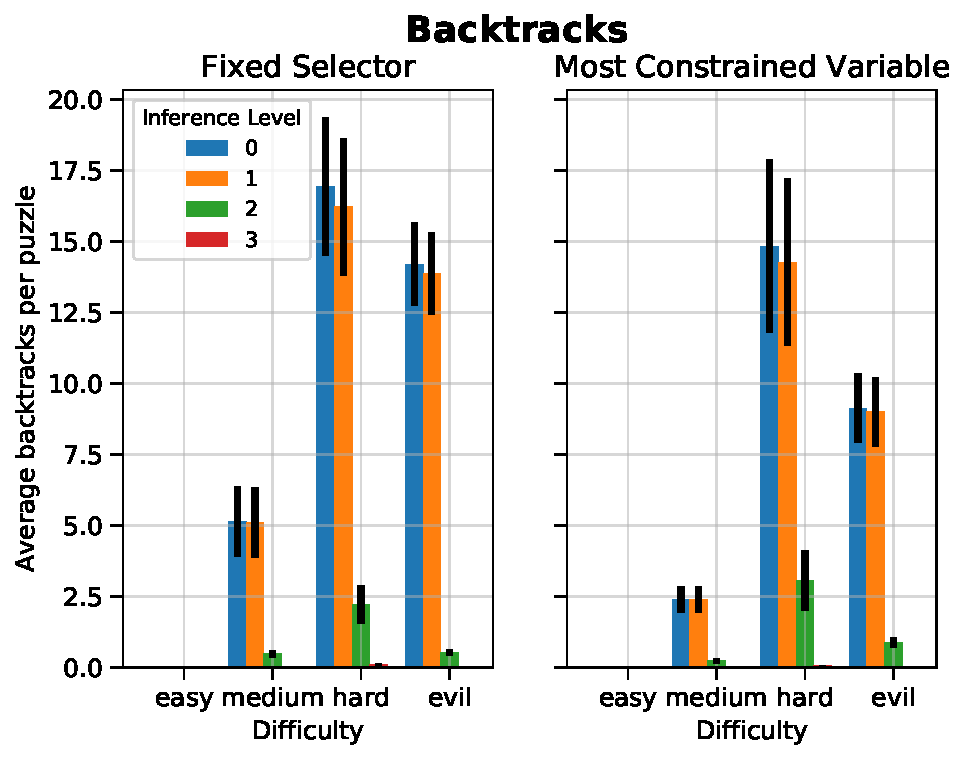
\includegraphics[width=\textwidth]{BackPerform}
	\caption{Average number of backtracks per puzzle and solver type.}	
	\label{f:BackPerf}
\end{figure}

Figure~\ref{f:BackPerf} shows the average number of backtracks performed by each problem difficulty and solver configuration, and illustrates the effect of the heuristic and high order inference methods on the necessity of backtracking.
It also shows that easy problems require only naked singles without backtracking to solve the problem.
In these problems, propagating constraints always leads to a variable with a single value in its domain.
Using doubles dramatically reduces the required backtracking steps for both heuristics on problems harder than easy.
Using triple inference rules almost eliminates the need for backtracking entirely. 
Only two problems, categorized hard require a single backtrack to be solved, and one of these problems requires a backtrack with the most constrained variable heuristic as well.

\begin{figure}[!h]
	\centering
	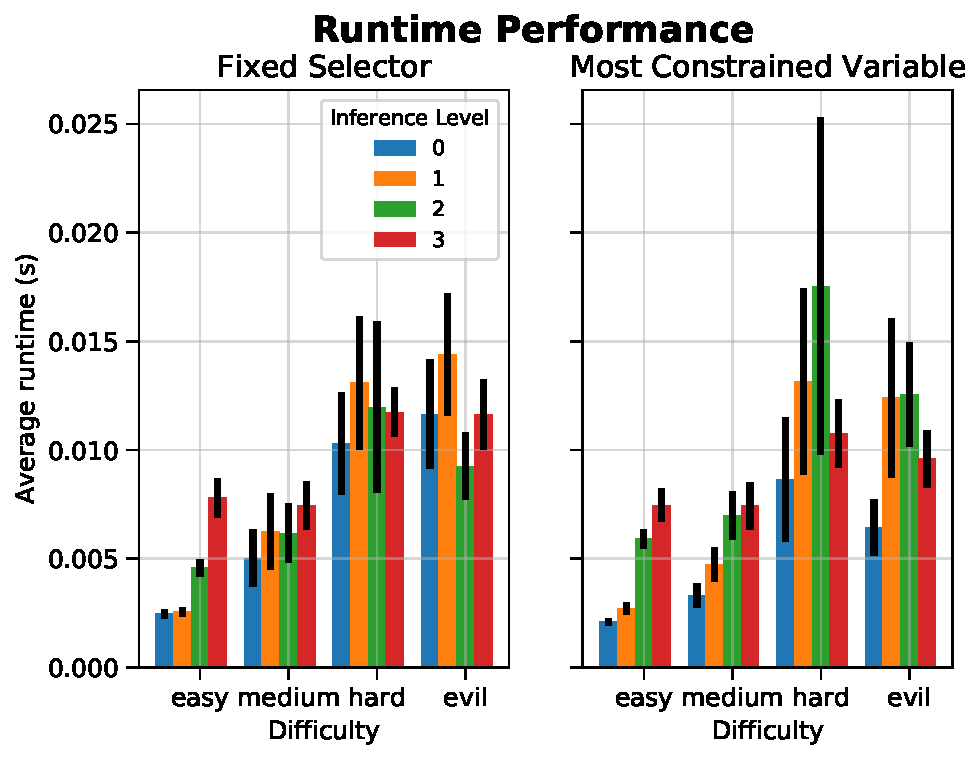
\includegraphics[width=\textwidth]{TimePerform}
	\caption{Time cost of solution per puzzle and solver type.}	
	\label{f:TimePerf}
\end{figure}

Reduced backtracking does not lead to increased performance.
Figure~\ref{f:TimePerf} shows the runtime for each solver; a particularly illustrative comparison is between the average backtracks and runtime result for hard problems using the most constrained variable heuristic allowing double but not triple inferences.
Figure~\ref{f:BackPerf} shows a roughly~$5\times$ reduction in backtracks by adding double inferences, yet the average runtime increases by about a third.
This is because inferences are about as costly as backtracks and must occur many times more often.

\section{Discussion}

Using the complexity of inference rules needed to solve a puzzle without backtracking is a good way to gauge the difficulty of a puzzle so the conjecture is roughly correct. 
Although, we do not observe that backtracking is an overwhelming drag on computational resources, the problems that require the most backtracking do tend to cost the most as seen in Figure~\ref{f:TimePerf}.
That is, increasing inference complexity to reduce backtracking does not effectively reduce runtime cost, but the categories that continue to require backtracking after further inferences are applied tend to take the most time.

Table~\ref{tab:boxct} shows the average number of boxes initially assigned with a single value, which is a proposed measure of difficulty.
This would seem to accurately reflect the difficulty of most problems, but miss out on important edge cases of difficulty.
Metaphorically, this is like saying that you can judge the time it takes to drive from city to city by the road mileage between them.
The \SI{120}{mi} from Cheyenne to Denver will probably take the predicted 2 hours, but that same distance from Philadelphia to New York will rarely pass so quickly.

\begin{table}[!ht]
	\centering
	\caption{Average number of initially assigned boxes}
	\label{tab:boxct}
	\begin{tabular}{||c c c c c||} 
		\hline
		& Easy & Medium & Hard & Evil \\ [0.5ex] 
		\hline
		Avg number & 34.7 & 29.0 & 26.3 & 26.1 \\ [1ex] 
		\hline
	\end{tabular}
\end{table}

The naked doubles and triple rules were effective, eliminating backtracking entirely for most problems. 
This means that in reality a user would not have to make an educated guess for a slot: the assignment step of backtracking search. 
This makes sense because a sudoku problem should be solvable with just constraint propagation and a set of rules even if the rules are more sophisticated than the naked triples.
However, a puzzle creator can easily amuse (or annoy) a solver by forcing them to perform a backtracking search, which translates to guessing squares and values and saving those guesses to change them later if they fail.

All easy problems were solved without backtracking or inference beyond naked singles. Once double inference rules were added, most medium problems (19 out of 21) could be solved without backtracking.
Using hidden singles does seem to mildly diminish backtracking, but also increases time cost.

\end{document}
